% !TEX program = xeLaTeX

\documentclass[12pt, a4paper, twoside]{article}
\usepackage[margin=1in]{geometry}
% support for CJK
\usepackage{xeCJK}
% support for graphics
\usepackage{graphicx}
% support for colors
\usepackage{xcolor}
\definecolor{dkgreen}{rgb}{0,0.6,0}
\definecolor{gray}{rgb}{0.5,0.5,0.5}
\definecolor{mauve}{rgb}{0.58,0,0.82}
% math packages
\usepackage{amsmath, amsthm, amssymb, bm}
% hyper references
\usepackage{hyperref}
\hypersetup{colorlinks=true, urlcolor=blue, linkcolor=blue, citecolor=blue}
% scientific units
\usepackage[separate-uncertainty = true]{siunitx}
\DeclareSIUnit\pixel{px}
% typesetting chemistry
\usepackage{mhchem}
% citations and references
% \usepackage[style=apa, backend=biber, sorting=nyt]{biblatex}
% additional symbols
\usepackage{gensymb}
\usepackage{textcomp}
% indent first paragraphs
\usepackage{indentfirst}
% ordinal numbers
\usepackage[super]{nth}
% more formatting for tables
\usepackage{multirow, makecell}
% typesetting program codes
\usepackage{listings}
\lstdefinestyle{python}{frame=tb,
  language=Python,
  aboveskip=3mm,
  belowskip=3mm,
  showstringspaces=false,
  columns=flexible,
  basicstyle={\small\ttfamily},
  numbers=left,
  numberstyle=\tiny\color{gray},
  keywordstyle=\color{blue},
  commentstyle=\color{dkgreen},
  stringstyle=\color{mauve},
  breaklines=true,
  breakatwhitespace=true,
  escapeinside=``,
  tabsize=4,
  extendedchars=false
}
\lstdefinestyle{output}{
  language=,
  basicstyle=\ttfamily,
  columns=fullflexible,
  breaklines=true,
  keepspaces=true,
  showstringspaces=false,
  frame=single,
  xleftmargin=5pt,
  xrightmargin=5pt,
}
\lstset{style=python}
\usepackage{tikz}
\usetikzlibrary{arrows.meta}
\usepackage{subcaption}

\title{A Brief Documentation of \texttt{obfusimg}}
\author{\_\_roselle\_\_, pigeon.hannah}

\makeatletter
\let\thetitle\@title
\let\theauthor\@author
\makeatother
\usepackage{fancyhdr}
\fancyhead[RO,LE]{\theauthor}
\fancyhead[LO,RE]{\thetitle}
\pagestyle{fancy}

% \addbibresource{citations.bib}

\begin{document}

\maketitle

\begin{abstract}
    The \texttt{obfusimg} application offers multiple algorithms that obfuscates images by shuffling the pixels of the image in a deterministic and revertible way. This document serves as a semi-technical manual for the C++ implementation of the application.
\end{abstract}

\section{Introduction} \label{intro}

Invertible image obfuscation has a wide range of applications, from privacy-preserving image sharing (e.g. circumventing censorship) to reversible preprocessing in scientific and industrial imaging pipelines （e.g. benchmarking machine learning architectures with disrupted spatial correlation).

A relatively straightforward approach to obfuscation is by rearranging all the pixels in a given image. Each pixels is moved to a unique new position following a certain method such that the output is an image of the same dimensions (width, lengths, number of channels) but hardly recognizable (see Figure~\ref{fig:rearranging_pixels_is_effective}).

\begin{figure}[b!]
    \centering
    \begin{subfigure}[t]{0.5\textwidth}
        \centering
        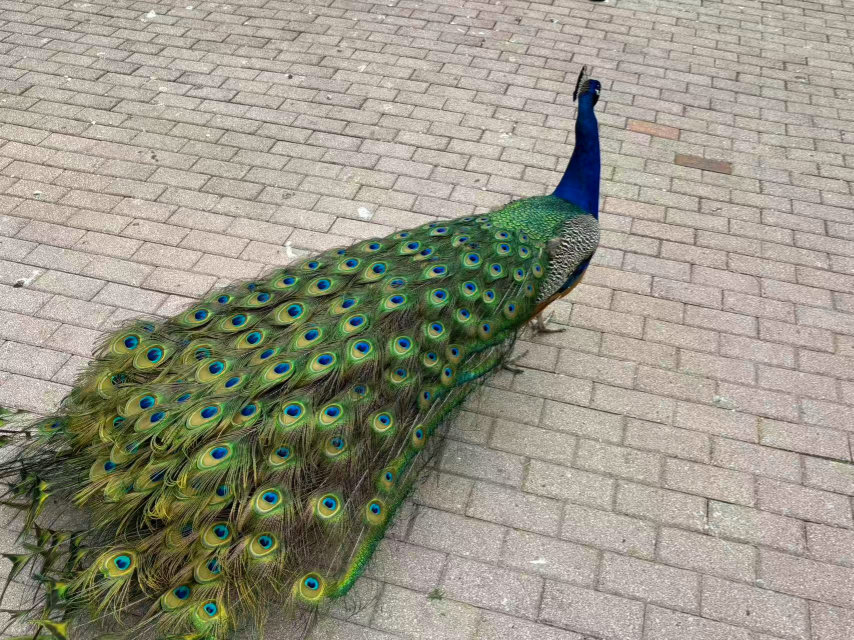
\includegraphics[width=.7\textwidth]{figures/demo_peacock.jpg}
        \caption{An image of a peacock (courtesy of mnrva).}
    \end{subfigure}%
    ~
    \begin{subfigure}[t]{0.5\textwidth}
        \centering
        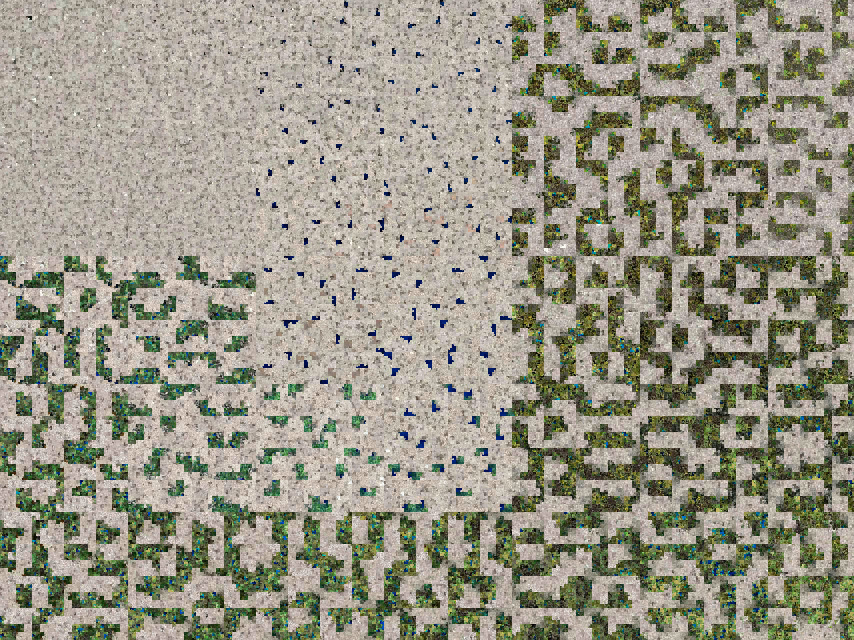
\includegraphics[width=.7\textwidth]{figures/demo_peacock_out.jpg}
        \caption{Peacock with all pixels rearranged.}
    \end{subfigure}
    \caption{The peacock in a demo image becomes unrecognizable after all the pixels are rearranged. State-of-the-art LLM's cannot reliably identify the subject of the obfuscated image (tested on ChatGPT 5.2 Thinking extended).}
    \label{fig:rearranging_pixels_is_effective}    
\end{figure}

The application \texttt{obfusimg} implements various algorithms that generate this method for pixel-rearrangement. In particular, the modest computation cost associated with these algorithms allow users to run the application on any reasonable local device meaning that no information needs to be transmitted through internet prior to obfuscation.

\section{Mathematical model of an image and obfuscation}

Let an image have width $w$ \si{\pixel}, height $h$ \si{\pixel}, and $c$ channels (typically, $c = 3$ for \texttt{jpeg} files with RGB channels and $c = 4$ for \texttt{png} files with RGB and Alpha channels). We identify the image with a $1$-dimensional array
\begin{equation}
    A = \bigl(a_0, a_1 \ldots, a_{w h - 1}\bigr)
\end{equation}
where each $a_i$ stores all $c$ channel values of one pixel (typically, each channel value is an integer $0 \leq n \leq 255$). Here, we use row-major indexing: if a pixel has coordinates $(x, y)$ in the original image with
\begin{equation}
    0 \leq x < w, \qquad 0 \leq y < h,
\end{equation}
then its array index is
\begin{equation}
    i = i(x, y) = y w + x.
\end{equation}
Note that this simply means we read the pixels from left to right, and top to bottom. This process is reversible as long as we know the width (or height) of the image.

An obfuscation method by rearranging all pixels can then be defined as a permutation\footnote{A map $f\colon A \to A$ is called a permutation of $A$ if $f$ is bijective. Therefore, a permutation $f\colon A \to A$ necessarily attains a unique inverse $f^{-1}\colon A \to A$.}
\begin{equation}
    \sigma\colon \{0, 1, \ldots, w h - 1 \} \to \{0, 1, \ldots, w h - 1 \}
\end{equation}
and the obfuscated image is
\begin{equation}
    A' = \bigl(a_{\sigma(n)}\bigr)_n.
\end{equation}
In other words, the $n$\textsuperscript{th} pixel in the obfuscated image corresponds to the $\sigma(n)$\textsuperscript{th} pixel in the original image. By applying the inverse obfuscation method $\sigma^{-1}$ to $A'$, we get
\begin{equation}
    A'' = \bigl(a_{\sigma^{-1}(\sigma(n))}\bigr)_n = \bigl(a_{n}\bigr)_n = A
\end{equation}
and recover the original image.

\section{Obfuscation algorithms}

Each algorithm implemented in \texttt{obfusimg} is essentially a map
\begin{equation}
    \alpha\colon \mathcal{I} \times [0, 1) \to \mathcal{P}, (I, s) \mapsto \sigma
\end{equation}
where $\mathcal{I}$ is the set of all images, $\mathcal{P}$ is the set of all permutations of finite sets, $I = (w, h, c, A)$ is a user-input image, $s \in [0, 1)$ is a user-defined seed, and $\sigma$ is a permutation of the set $\{0, 1, \ldots, w h - 1\}$. In practice, $\alpha(I, s)$ almost never depends on $c$ and $A$ since $c$ has little variability and $A$ is prone to compression loss for \texttt{jpeg} files.

\subsection{G/Hilbert curves}

A Hilbert curve\footnote{Technically, we are using finite iterations of curves leading up to Hilbert curves. Hilbert curves, like Peano curves, are space filling curves and serve as examples of \emph{continuous} bijective maps from $[0, 1]$ to $[0, 1]^2$. This is surprising since $C^1$ images of lower-dimensional rectangles have zero Jordan measure.} (Gilbert curve) for a $2^n$-by-$2^n$ square is a ``continuous'' curve traveling via adjacent pixels through square with each pixel visited exactly once. By labeling the pixel indices with the corresponding steps, we effectively get a permutation
\begin{equation}
    h\colon \{0, 1, \ldots, 2^{2n} - 1\} \to \{0, 1, \ldots, 2^{2n} - 1\}, \text{step} \mapsto \text{pixel index at step}.
\end{equation}
Since Hilbert curves are limits of fractals, a simple recursion gives us the Hilbert curve for an arbitrary $n$.

A generalized Hilbert curve (Gilbert curve) for a $w$-by-$h$ rectangle is a generalized version of a Hilbert curve that is ``continuous'' and reaches each pixel exactly once (see Figure~\ref{fig:gilbert_curve}). Similarly, this curve defines get a permutation
\begin{equation}
    g\colon \{0, 1, \ldots, w h - 1\} \to \{0, 1, \ldots, w h - 1\}
\end{equation}
which we could use as our desired permutation $\sigma$.

\begin{figure}[t!]
\centering
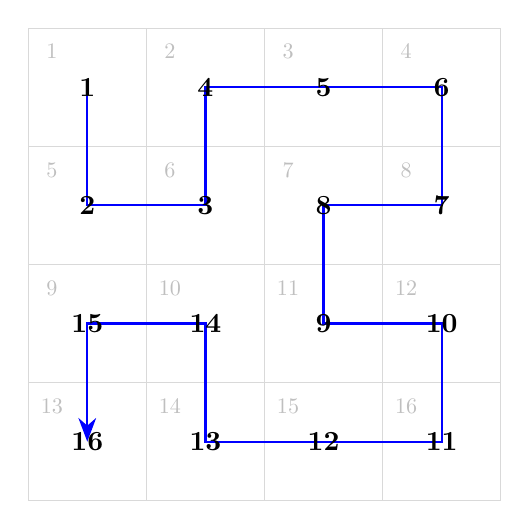
\begin{tikzpicture}[scale=1.5]
    % Draw the grid
    \draw[step=1cm, gray!30, thin] (0,0) grid (4,4);

    % Original pixel labeling (left-to-right, top-to-bottom)
    % Convention: (column, row) mapping to 1D index
    \foreach \y [evaluate=\y as \rowindex using int(4-\y)] in {1,2,3,4}
        \foreach \x [evaluate=\x as \colindex using int(\x-1)] in {1,2,3,4}
            \node[gray!50, scale=0.8] at (\x-0.8, \y-0.2) {\the\numexpr \rowindex*4 + \colindex\relax};

    % The Gilbert/Hilbert Path Coordinates for 4x4
    % Sequence: (0,0), (0,1), (1,1), (1,0), (2,0), (3,0), (3,1), (2,1), (2,2), (3,2), (3,3), (2,3), (1,3), (1,2), (0,2), (0,3)
    % Adjusted to grid centers (0.5 offset) and flipped Y for top-down
    \draw[thick, blue, -{Stealth[length=3mm]}] 
        (0.5, 3.5) -- (0.5, 2.5) -- (1.5, 2.5) -- (1.5, 3.5) -- 
        (2.5, 3.5) -- (3.5, 3.5) -- (3.5, 2.5) -- (2.5, 2.5) -- 
        (2.5, 1.5) -- (3.5, 1.5) -- (3.5, 0.5) -- (2.5, 0.5) -- 
        (1.5, 0.5) -- (1.5, 1.5) -- (0.5, 1.5) -- (0.5, 0.5);

    % Relabeling g(1)...g(16)
    \coordinate (P1)  at (0.5, 3.5); \node[font=\bfseries] at (P1) {1};
    \coordinate (P2)  at (0.5, 2.5); \node[font=\bfseries] at (P2) {2};
    \coordinate (P3)  at (1.5, 2.5); \node[font=\bfseries] at (P3) {3};
    \coordinate (P4)  at (1.5, 3.5); \node[font=\bfseries] at (P4) {4};
    \coordinate (P5)  at (2.5, 3.5); \node[font=\bfseries] at (P5) {5};
    \coordinate (P6)  at (3.5, 3.5); \node[font=\bfseries] at (P6) {6};
    \coordinate (P7)  at (3.5, 2.5); \node[font=\bfseries] at (P7) {7};
    \coordinate (P8)  at (2.5, 2.5); \node[font=\bfseries] at (P8) {8};
    \coordinate (P9)  at (2.5, 1.5); \node[font=\bfseries] at (P9) {9};
    \coordinate (P10) at (3.5, 1.5); \node[font=\bfseries] at (P10) {10};
    \coordinate (P11) at (3.5, 0.5); \node[font=\bfseries] at (P11) {11};
    \coordinate (P12) at (2.5, 0.5); \node[font=\bfseries] at (P12) {12};
    \coordinate (P13) at (1.5, 0.5); \node[font=\bfseries] at (P13) {13};
    \coordinate (P14) at (1.5, 1.5); \node[font=\bfseries] at (P14) {14};
    \coordinate (P15) at (0.5, 1.5); \node[font=\bfseries] at (P15) {15};
    \coordinate (P16) at (0.5, 0.5); \node[font=\bfseries] at (P16) {16};
\end{tikzpicture}
\caption{An example of a Gilbert curve for a $4$-by-$4$ rectangle. The gray numerals represent the original indices and the black numerals represent the rearranged indices. In other words, $g(\text{black}) = \text{gray}$. Note that the Gilbert curve here is slightly different from the actual Gilbert curve implemented in \texttt{gilbert\_curve.cpp}.}
\label{fig:gilbert_curve}
\end{figure}

A na\"{i}ve attempt at the problem of computing Gilbert curves suggests ``padding'' the $w$-by-$h$ rectangle to the smallest containing $2^n$-by-$2^n$ square, computing the Hilbert curve for that square, and truncating the parts of the curve outside of the rectangle. However, this is computationally inefficient as we will usually waste over half of our computation resources computing the curve outside of the rectangle. Here we use two advanced methods.

\subsubsection{Compact Gilbert curves}

This method\footnote{See ``Compact Hilbert indices: Space-filling curves for domains with unequal side lengths.'' Available at \url{https://doi.org/10.1016/j.ipl.2007.08.034}.} suggested by Chris H. Hamilton and Andrew Rau-Chaplin computes
\begin{equation}
    w^* = \lceil \log_2(w) \rceil, \qquad h^* = \lceil \log_2(h) \rceil
\end{equation}
as the number of bits ($0$ or $1$) needed to represent an $x$ and $y$ index respectively. The method takes a point $(x, y)$, starts with the coarsest (highest) bit level, determines the quadrant of the point in the current bit level and setting the corresponding bit(s), descends into a lower level, and repeats.

At the end of the process, one obtains an index $0 \leq C(x, y) \leq 2^{w^* + h^*} - 1$ that describes the position of the point on a Gilbert curve. By computing $\tilde{C}(x, y)$ for all $0 \leq x < w$ and $0 \leq y < h$, we obtain the \emph{unnormalized} compact Gilbert function
\begin{equation}
    C\colon \{0, 1, \ldots, w h - 1\} \to \{0, 1, \ldots, 2^{w^* + h^*} - 1\}.
\end{equation}
that is injective but usually not surjective. We normalize $C$ by ranking the outputs to get the \emph{normalized} compact Gilbert function
\begin{equation}
    \tilde{g}\colon N = \{0, 1, \ldots, w h - 1\} \to N, i \mapsto \text{rank of $C(i)$ in $C(N)$}.
\end{equation}
This $\tilde{g}$ is such that $\tilde{g}(i)$ is the position of the point with index $i$ on the ``truncated curve.'' By taking the inverse of $\tilde{g}$, we get
\begin{equation}
    g\colon \{0, 1, \ldots, w h - 1\} \to \{0, 1, \ldots, w h - 1\}, i \mapsto \tilde{g}^{-1}(i)
\end{equation}
which gives the index of the $i$\textsuperscript{th} point on the curve. This $g$ is our desired permutation $\sigma$.

\subsubsection{Exact Gilbert curves}

This method\footnote{See \url{https://github.com/jakubcerveny/gilbert/}.} suggested by Jakub Červený computes a curve that travels exclusively in the $w$-by-$h$ rectangle by recursively splitting a rectangle into three regions following a U-shaped path. Note that in particular cases, a diagonal move may be used. This method gives us a \emph{normalized} exact Gilbert function
\begin{equation}
    g\colon \{0, 1, \ldots, w h - 1\} \to \{0, 1, \ldots, w h - 1\}
\end{equation}
which gives the index of the $i$\textsuperscript{th} point on the curve.

Following a popular tool ``小番茄图片混淆''\footnote{See \url{https://xfqtphx.netlify.app/}.}, we do not use this $g$ directly as our permutation for this case. Instead, we rearrange our pixels by shifting each pixel along the exact Gilbert curve by an offset of
\begin{equation}
    k = \Bigl\lfloor \frac{\sqrt{5} - 1}{2} h w \Bigr\rceil = \Bigl\lfloor \frac{h w}{\varphi} \Bigr\rceil.
\end{equation}
This means that the new pixel at index $j$ which is originally the $g^{-1}(j)$\textsuperscript{th} point on the curve should be the $(g^{-1}(j) - k)$\textsuperscript{th} point on the curve after the shift. Since $g$ is bijective, $j = g(i)$ for some $i$. Our desired permutation is then
\begin{equation}
    \sigma\colon \{0, 1, \ldots, w h - 1\} \to \{0, 1, \ldots, w h - 1\}, g(i) \mapsto g(\overline{i - k})
\end{equation}
where $\overline{i - k}$ is understood to be $\bmod \; h w$. Notice that the permutation is well-defined since $g$ is bijective.

\subsection{Chaotic systems}

If we simply want a highly noise-like but reproducible $\sigma$ (lava lamps in Cloudflare's SF office generate very noisy data, but there is no hope of inverting the permutation afterwards), we may look at chaotic systems. very loosely\footnote{Strictly speaking, there are various rigorous mathematical definitions for chaotic systems. A most classical one is Devaney chaos defined for continuous functions $f\colon X \to X$ on a metric space $(X, d)$. Such a function $f$ is Devaney chaotic if it is topologically transitive, has dense periodic points, and has sensitive dependence on initial conditions. However, let us reserve that for a math course.}, we characterize chaotic systems by the following properties:
\begin{itemize}
    \item The system evolves deterministically. That is, there is a well-defined function $f$ such that $x_{n + 1} = f(x_n)$ always.
    \item The system, with any initial state, can evolve to any region given enough time.
    \item The system is sensitive to initial conditions. That is, two starting points close to each other can evolve in drastically different ways.
\end{itemize}

There are many simple functions $f\colon I \subseteq \mathbb{R} \to \mathbb{R}$ that exhibit chaotic behavior. For example, the logistic map $L(x) = r x (1 - x)$ for $r \lesssim 4$, the tent map $T(x) = \mu \min\{x, 1 - x\}$ for $\mu \in (1, 2)$ (see Figure~\ref{fig:tent_map}), and the doubling map $D(x) = 2 x \pmod 1$ can all be used to simulate chaos.

\begin{figure}[b!]
    \centering
    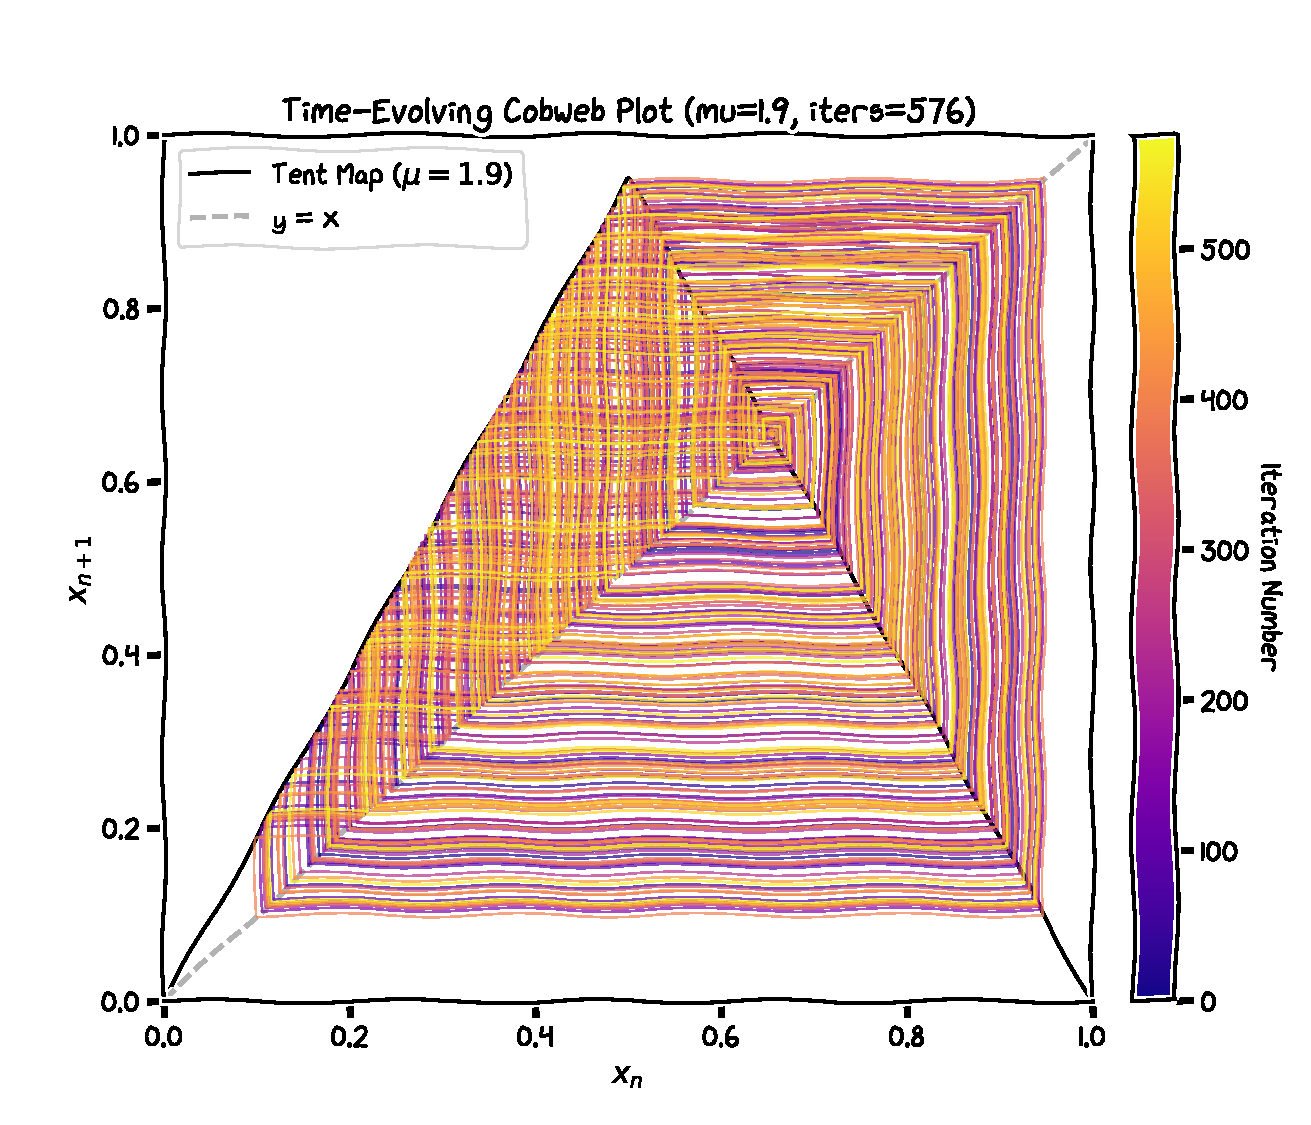
\includegraphics[width=0.6\linewidth]{figures/tent_map.pdf}
    \caption{Evolution of the tent map with $\mu = 1.9$ and $x_0 = 0.7$ after ${24}^2$ iterations.}
    \label{fig:tent_map}
\end{figure}

Assume a chaotic map $f\colon I \subseteq \mathbb{R} \to \mathbb{R}$. A user-defined seed $s$ sets the initial condition $x_0 = s$. For $0 \leq i < w h - 1$, we compute
\begin{equation}
    x_{i + 1} = f(x_i).
\end{equation}
This gives us a noise-like array $(x_n)_n$. We may rank the $x_n$'s by sorting, using the indices $n$'s to break ties if necessary. This gives us the desired permutation
\begin{equation}
    \sigma\colon \{0, 1, \ldots, w h - 1\} \to \{0, 1, \ldots, w h - 1\}, i \mapsto \text{$n$ such that $x_n$ has rank $i$}.
\end{equation}

\subsubsection{Tent map}

We implement the tent map as
\begin{equation}
    T_\mu\colon [0, 1] \to [0, 1], x \mapsto 
    \begin{cases}
        \mu x & x < 1/2, \\
        \mu (1 - x) & x \geq 1/2
    \end{cases}
\end{equation}
for $0 < \mu \leq 2$. This map is highly chaotic for $\mu = 2$. However, in an actual C++ implementation multiplication by $2$ is effectively a bit-wise left shift. With finite precision, we will loose all bits after approximately 53 iterations. Therefore, we set $\mu = 1.9999$.

\pagebreak

\appendix

\section*{Appendices}

\setcounter{figure}{0}
\renewcommand{\thefigure}{A\arabic{figure}}

\setcounter{table}{0}
\renewcommand{\thetable}{A\arabic{table}}

\section{header file for permutations module}

\lstinputlisting[language=C++]{../permutation.h}

\clearpage

\section{header file for Gilbert curves module}

\lstinputlisting[language=C++]{../gilbert_curve.h}

\clearpage

\section{header file for chaotic systems module}

\lstinputlisting[language=C++]{../chaos.h}

\end{document}